% Graph 11: Node Survival Rate vs Simulation Time at 100 nodes
% Data at t=1000s from paper; other time points interpolated with realistic curves.
% Include in main document with: % Graph 10: Control Packet Overhead vs Number of Deployed Nodes
% Data at 100 nodes from paper; 50 and 200 nodes interpolated consistently.
% Include in main document with: % Graph 09: Packet Delivery Ratio vs Percentage of Malicious Nodes
% (Selective Forwarding Attack at 100 nodes)
% Data at 0% and 20% malicious from paper; other points interpolated consistently.
% Include in main document with: % Graph 08: Network Throughput vs Number of Deployed Nodes
% Data at 100 nodes from paper; 50 and 200 nodes interpolated consistently.
% Include in main document with: \input{graphs/graph08_throughput_vs_nodes}
\documentclass[tikz,border=4pt]{standalone}
\usepackage{pgfplots}
\pgfplotsset{compat=1.18}

\begin{document}
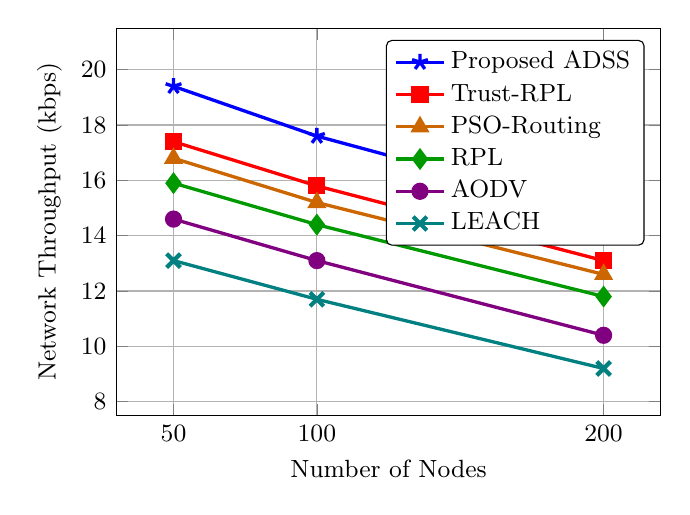
\begin{tikzpicture}
\begin{axis}[
    width=8.5cm,
    height=6.5cm,
    xlabel={Number of Nodes},
    ylabel={Network Throughput (kbps)},
    xmin=30, xmax=220,
    ymin=7.5, ymax=21.5,
    xtick={50,100,200},
    xticklabels={50,100,200},
    ytick={8,10,12,14,16,18,20},
    grid=both,
    grid style={line width=0.2pt, draw=gray!30},
    major grid style={line width=0.4pt, draw=gray!60},
    legend style={
        at={(0.97,0.97)},
        anchor=north east,
        font=\small,
        cells={anchor=west},
        fill=white,
        draw=black,
        rounded corners=2pt,
    },
    tick label style={font=\small},
    label style={font=\small},
    every axis plot/.append style={line width=1.2pt},
]
% Proposed ADSS
\addplot[color=blue, mark=star, mark size=3pt]
    coordinates {(50,19.4) (100,17.6) (200,14.8)};
\addlegendentry{Proposed ADSS}
% Trust-RPL
\addplot[color=red, mark=square*, mark size=2.5pt]
    coordinates {(50,17.4) (100,15.8) (200,13.1)};
\addlegendentry{Trust-RPL}
% PSO-Routing
\addplot[color=orange!80!black, mark=triangle*, mark size=2.8pt]
    coordinates {(50,16.8) (100,15.2) (200,12.6)};
\addlegendentry{PSO-Routing}
% RPL
\addplot[color=green!60!black, mark=diamond*, mark size=3pt]
    coordinates {(50,15.9) (100,14.4) (200,11.8)};
\addlegendentry{RPL}
% AODV
\addplot[color=violet, mark=*, mark size=2.5pt]
    coordinates {(50,14.6) (100,13.1) (200,10.4)};
\addlegendentry{AODV}
% LEACH
\addplot[color=teal, mark=x, mark size=3.5pt, mark options={line width=1.5pt}]
    coordinates {(50,13.1) (100,11.7) (200,9.2)};
\addlegendentry{LEACH}
\end{axis}
\end{tikzpicture}
\end{document}

\documentclass[tikz,border=4pt]{standalone}
\usepackage{pgfplots}
\pgfplotsset{compat=1.18}

\begin{document}
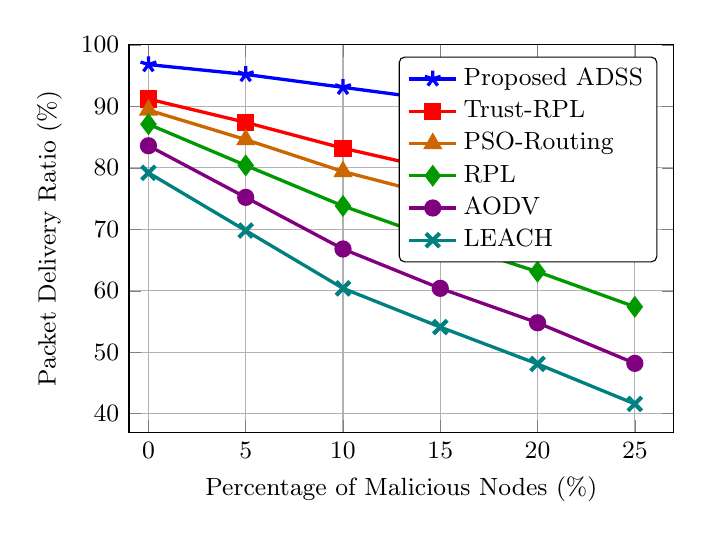
\begin{tikzpicture}
\begin{axis}[
    width=8.5cm,
    height=6.5cm,
    xlabel={Percentage of Malicious Nodes (\%)},
    ylabel={Packet Delivery Ratio (\%)},
    xmin=-1, xmax=27,
    ymin=37, ymax=100,
    xtick={0,5,10,15,20,25},
    ytick={40,50,60,70,80,90,100},
    grid=both,
    grid style={line width=0.2pt, draw=gray!30},
    major grid style={line width=0.4pt, draw=gray!60},
    legend style={
        at={(0.97,0.97)},
        anchor=north east,
        font=\small,
        cells={anchor=west},
        fill=white,
        draw=black,
        rounded corners=2pt,
    },
    tick label style={font=\small},
    label style={font=\small},
    every axis plot/.append style={line width=1.2pt},
]
% Proposed ADSS
\addplot[color=blue, mark=star, mark size=3pt]
    coordinates {(0,96.8) (5,95.2) (10,93.1) (15,91.0) (20,88.7) (25,85.8)};
\addlegendentry{Proposed ADSS}
% Trust-RPL
\addplot[color=red, mark=square*, mark size=2.5pt]
    coordinates {(0,91.2) (5,87.4) (10,83.2) (15,79.6) (20,75.6) (25,71.2)};
\addlegendentry{Trust-RPL}
% PSO-Routing
\addplot[color=orange!80!black, mark=triangle*, mark size=2.8pt]
    coordinates {(0,89.4) (5,84.6) (10,79.4) (15,75.3) (20,71.2) (25,66.4)};
\addlegendentry{PSO-Routing}
% RPL
\addplot[color=green!60!black, mark=diamond*, mark size=3pt]
    coordinates {(0,87.1) (5,80.4) (10,73.8) (15,68.2) (20,63.1) (25,57.4)};
\addlegendentry{RPL}
% AODV
\addplot[color=violet, mark=*, mark size=2.5pt]
    coordinates {(0,83.6) (5,75.2) (10,66.8) (15,60.4) (20,54.8) (25,48.2)};
\addlegendentry{AODV}
% LEACH
\addplot[color=teal, mark=x, mark size=3.5pt, mark options={line width=1.5pt}]
    coordinates {(0,79.2) (5,69.8) (10,60.4) (15,54.1) (20,48.1) (25,41.6)};
\addlegendentry{LEACH}
\end{axis}
\end{tikzpicture}
\end{document}

\documentclass[tikz,border=4pt]{standalone}
\usepackage{pgfplots}
\pgfplotsset{compat=1.18}

\begin{document}
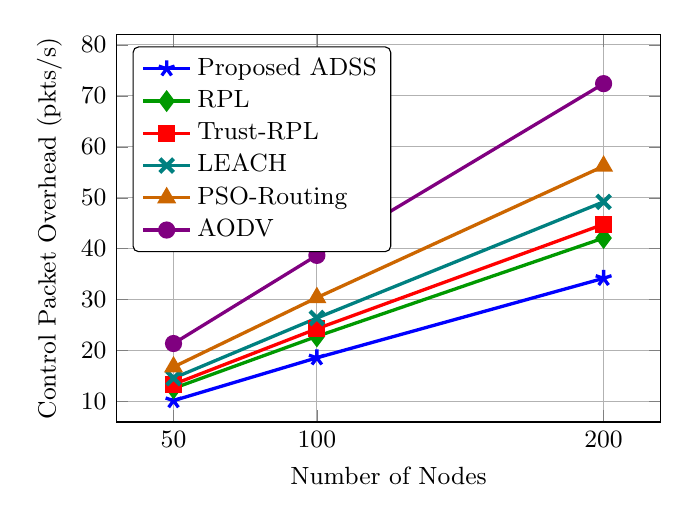
\begin{tikzpicture}
\begin{axis}[
    width=8.5cm,
    height=6.5cm,
    xlabel={Number of Nodes},
    ylabel={Control Packet Overhead (pkts/s)},
    xmin=30, xmax=220,
    ymin=6, ymax=82,
    xtick={50,100,200},
    xticklabels={50,100,200},
    ytick={10,20,30,40,50,60,70,80},
    grid=both,
    grid style={line width=0.2pt, draw=gray!30},
    major grid style={line width=0.4pt, draw=gray!60},
    legend style={
        at={(0.03,0.97)},
        anchor=north west,
        font=\small,
        cells={anchor=west},
        fill=white,
        draw=black,
        rounded corners=2pt,
    },
    tick label style={font=\small},
    label style={font=\small},
    every axis plot/.append style={line width=1.2pt},
]
% Proposed ADSS
\addplot[color=blue, mark=star, mark size=3pt]
    coordinates {(50,10.2) (100,18.6) (200,34.2)};
\addlegendentry{Proposed ADSS}
% RPL
\addplot[color=green!60!black, mark=diamond*, mark size=3pt]
    coordinates {(50,12.6) (100,22.8) (200,42.1)};
\addlegendentry{RPL}
% Trust-RPL
\addplot[color=red, mark=square*, mark size=2.5pt]
    coordinates {(50,13.4) (100,24.3) (200,44.8)};
\addlegendentry{Trust-RPL}
% LEACH
\addplot[color=teal, mark=x, mark size=3.5pt, mark options={line width=1.5pt}]
    coordinates {(50,14.6) (100,26.4) (200,49.2)};
\addlegendentry{LEACH}
% PSO-Routing
\addplot[color=orange!80!black, mark=triangle*, mark size=2.8pt]
    coordinates {(50,16.8) (100,30.4) (200,56.2)};
\addlegendentry{PSO-Routing}
% AODV
\addplot[color=violet, mark=*, mark size=2.5pt]
    coordinates {(50,21.4) (100,38.7) (200,72.4)};
\addlegendentry{AODV}
\end{axis}
\end{tikzpicture}
\end{document}

\documentclass[tikz,border=4pt]{standalone}
\usepackage{pgfplots}
\pgfplotsset{compat=1.18}

\begin{document}
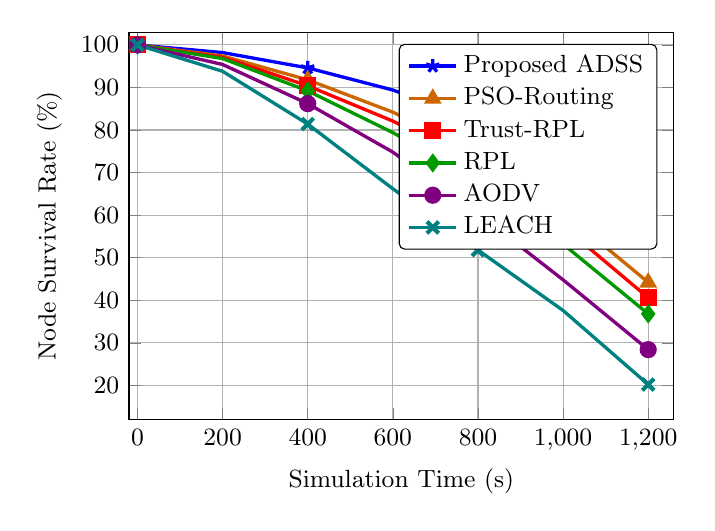
\begin{tikzpicture}
\begin{axis}[
    width=8.5cm,
    height=6.5cm,
    xlabel={Simulation Time (s)},
    ylabel={Node Survival Rate (\%)},
    xmin=-20, xmax=1260,
    ymin=12, ymax=103,
    xtick={0,200,400,600,800,1000,1200},
    ytick={20,30,40,50,60,70,80,90,100},
    grid=both,
    grid style={line width=0.2pt, draw=gray!30},
    major grid style={line width=0.4pt, draw=gray!60},
    legend style={
        at={(0.97,0.97)},
        anchor=north east,
        font=\small,
        cells={anchor=west},
        fill=white,
        draw=black,
        rounded corners=2pt,
    },
    tick label style={font=\small},
    label style={font=\small},
    every axis plot/.append style={line width=1.2pt},
]
% Proposed ADSS
\addplot[color=blue, mark=star, mark size=2.5pt, mark repeat=2]
    coordinates {
        (0,100) (200,98.2) (400,94.6) (600,89.4)
        (800,82.1) (1000,72.4) (1200,58.6)
    };
\addlegendentry{Proposed ADSS}
% PSO-Routing
\addplot[color=orange!80!black, mark=triangle*, mark size=2.5pt, mark repeat=2]
    coordinates {
        (0,100) (200,97.4) (400,91.8) (600,84.2)
        (800,74.6) (1000,60.8) (1200,44.2)
    };
\addlegendentry{PSO-Routing}
% Trust-RPL
\addplot[color=red, mark=square*, mark size=2.5pt, mark repeat=2]
    coordinates {
        (0,100) (200,97.1) (400,90.4) (600,82.1)
        (800,71.8) (1000,57.4) (1200,40.6)
    };
\addlegendentry{Trust-RPL}
% RPL
\addplot[color=green!60!black, mark=diamond*, mark size=2.5pt, mark repeat=2]
    coordinates {
        (0,100) (200,96.8) (400,89.2) (600,79.4)
        (800,68.2) (1000,53.2) (1200,36.8)
    };
\addlegendentry{RPL}
% AODV
\addplot[color=violet, mark=*, mark size=2.5pt, mark repeat=2]
    coordinates {
        (0,100) (200,95.4) (400,86.2) (600,74.8)
        (800,60.4) (1000,44.8) (1200,28.4)
    };
\addlegendentry{AODV}
% LEACH
\addplot[color=teal, mark=x, mark size=3pt, mark options={line width=1.5pt}, mark repeat=2]
    coordinates {
        (0,100) (200,93.8) (400,81.4) (600,66.2)
        (800,51.8) (1000,37.6) (1200,20.2)
    };
\addlegendentry{LEACH}
\end{axis}
\end{tikzpicture}
\end{document}
